\chapter{Задача о рюкзаке}

Имеется рюкзак грузоподъемностью S = 20. Требуется заполнить его грузом, состоящим из предметов N = 6 различных типов таким образом, чтобы стоимость (ценность) всего груза была максимальной.

\begin{center}
    \begin{tabular}{|a | c | c | c | c | c | c|} 
         \hline
         \rowcolor{LightGray}
            С (предметы) & 1 & 2 & 3 & 4 & 5 & 6\\
        \hline
            Р (вес) & 9 & 5 & 8 & 7 & 4 & 6 \\
         \hline
            V (цена) & 12 & 9 & 14 & 10 & 16 & 8 \\
         \hline
    \end{tabular}
\end{center}

\begin{center}
    {\bf
    Решение:}
\end{center}

\begin{center}
    $W(x) = \displaystyle \sum_{i=1}^{6} x_{i}V_{i} \rightarrow max$\\
    $\displaystyle \sum_{i=1}^{6} x_{i}P_{i} \le 20, x_{i} = 0, 1,...$ - целочисленное\\
\end{center}

\subsection*{1)}
$W_1 (C)=\underset{0\le x_1 \le [\frac{25}{9}]}{max}\{x_1\cdot 12\}, x_1=0,1,2$

\begin{center}
    \begin{tabular}{|a|c|c|c|}
    \hline 
    C & 0-8 & 9-17 & 18-20\\ \hline
    $W_1 (C)$ & 0 & 12 & 24\\ \hline
    $x_1$ & 0 & 1 & 2\\ \hline
    \end{tabular}
\end{center}


\subsection*{2)}
$W_2 (S)=\underset{0\le x_2 \le [\frac{C}{5}]}{max}\{x_2\cdot 9 + W_1(C-x_2\cdot 5)\}, x_2=0,1,2,3,4$

\begin{center}
    \small
    \begin{tabular}{|a|c|c|c|c|c|c|c|c|}
    \hline 
    C & 0-4 & 5-8 & 9 & 10-13 & 14 & 15-18 & 19 & 20\\ \hline
    $W_2 (C)$ & 0 & 9 & 12 & 18 & 21 & 27 & 30 & 36 \\ \hline
    $x_2$ & 0 & 1 & 0 & 2 & 1 & 3 & 2 & 4 \\ \hline
    \end{tabular}
\end{center}



\subsection*{3)}
$W_3 (S)=\underset{0\le x_3 \le [\frac{C}{8}]}{max}\{x_3\cdot 14+W_2(C-x_3\cdot 8)\}, x_3=0,1,2$


\begin{flushleft}
    \small
    \begin{tabular}{|a|c|c|c|c|c|c|c|c|c|}
    \hline 
    C & 0-4 & 5-7 & 8-9 & 10-12 & 13-14 & 15 & 16-17 & 18-19 & 20\\ \hline
    $W_3 (C)$ & 0 & 9 & 14 & 18 & 23 & 27 & 28 & 32 & 36 \\ \hline
    $x_3$ & 0 & 0 & 1 & 0 & 1 & 0 & 2 & 1 & 0\\ \hline
    \end{tabular}
\end{flushleft}


\subsection*{4)}
$W_4 (S)=\underset{0\le x_4 \le [\frac{C}{7}]}{max}\{x_4\cdot 10+W_3(C-x_4\cdot 7)\}, x_4=0,1,2$

\begin{flushleft}
    \small
    \begin{tabular}{|a|c|c|c|c|c|c|c|c|c|c|c|}
    \hline 
    C & 0-4 & 5-6 & 7 & 8-9 & 10-11 & 12 & 13-14 & 15 & 16-17 & 18-19 & 20\\ \hline
    $W_3 (C)$ & 0 & 9 &  10& 14 & 18 & 19 & 23 & 27 & 28 & 32 & 36 \\ \hline
    $x_3$ & 0 & 0 & 1 & 0 & 0 & 1 & 0 & 0 & 0 & 0 & 0\\ \hline
    \end{tabular}
\end{flushleft}


\subsection*{5)}
$W_5 (S)=\underset{0\le x_5 \le [\frac{C}{4}]}{max}\{x_5\cdot 16+W_4(C-x_5\cdot 4)\}, x_5=\overline{0,5}$

\begin{flushleft}
    \small
    \begin{tabular}{|a|c|c|c|c|c|c|}
    \hline 
    C & 0-3 & 4-7 & 8-11 & 12-15 & 16-19 & 20 \\ \hline
    $W_3 (C)$ & 0 & 16 & 32 & 48 & 64 & 80 \\ \hline
    $x_3$ & 0 & 1 & 2 & 3 & 4 & 5 \\ \hline
    \end{tabular}
\end{flushleft}



\subsection*{6)}
$W_6 (S)=\underset{0\le x_6 \le [\frac{C}{6}]}{max}\{x_6\cdot 8+W_5(C-x_6\cdot 6)\}, x_5=\overline{0,3}$

\begin{flushleft}
    \small
    \begin{tabular}{|a|c|c|c|c|c|c|}
    \hline 
    C & 0-3 & 4-7 & 8-11 & 12-15 & 16-19 & 20 \\ \hline
    $W_3 (C)$ & 0 & 16 & 32 & 48 & 64 & 80 \\ \hline
    $x_3$ & 0 & 0 & 0 & 0 & 0 & 0 \\ \hline
    \end{tabular}
\end{flushleft}

Максимальная стоимость груза равна:$W_6(20)=80$\\
$
W_6(20)=80 \text{ при } x_6=0 \implies x_6^o=0\implies\\
W_6(20)=0\cdot 8 + W_5(20-0\cdot 6)=80\implies W_5(20)=80\implies\\
W_5(20)=80 \text{ при } x_5=5 \implies x_5^o=5\implies\\
W_5(20)=5\cdot 16 + W_4(20-5\cdot 4)=80\implies W_4(0)=0\implies\\
W_4(0)=0 \text{ при } x_4=0 \implies x_4^o=0\implies\\
W_3(0)=W_2(0)=W_1(0)=0 \text{ при } x_3= x_2 = x_1=0 \implies \\
x_3^o=x_2^o=x_1^o=0
$

{\bfОтвет:} максимальная стоимость груза равна 80, \\
опорный план: $x^0 = (0, 0, 0, 0, 5, 0)$

{\bfКод программы на Python для решения задачи о рюкзаке}

\begin{lstlisting}
    weights = [9, 5, 8, 7, 4, 6]
    values = [12, 9, 14, 10, 16, 8]
    capacity = 20
    
    max_profit = 0
    A = [0] * 6
    optimal = " "
    
    while A [0] * weights [0] <= capacity :
        A [1] = 0
        profit = A [0] * values [0]
        while A [1] * weights [1] <= capacity - A [0] * weights [0]:
            A [2] = 0
            while ( A [2] * weights [2] <= capacity - A [0] * weights [0] - A [1] * weights [1]) :
                A [3] = 0
                while ( A [3] * weights [3] <= capacity - A [0] * weights [0] - A [1] * weights [1] - A [2] * weights [2]) :
                    A [4] = 0
                    while ( A [4] * weights [4] <= capacity - A [0] * weights [0] - A [1] * weights [1] - A [2] * weights [2] - A [3] * weights [3]) :
                        A [5] = 0
                        while ( A [5] * weights [5] <= capacity - A [0] * weights [0] - A [1] * weights [1] - A [2] * weights [2] - A [3] * weights [3] - A [4] * weights [4]) :
                            profit = A [0] * values [0]
                            profit += A [1] * values [1]
                            profit += A [2] * values [2]
                            profit += A [3] * values [3]
                            profit += A [4] * values [4]
                            profit += A [5] * values [5]
                            if profit > max_profit :
                                max_profit = profit
                                optimal = str ( A [0]) + " , "
                                optimal += str ( A [1]) + " , "
                                optimal += str ( A [2]) + " , "
                                optimal += str ( A [3]) + " , "
                                optimal += str ( A [4]) + " , "
                                optimal += str ( A [5])
                            A [5] += 1
                        A [4] += 1
                    A [3] += 1
                A [2] += 1
            A [1] += 1
        A [0] += 1
    
    
    print ( " Max cost : " + str ( max_profit ) )
    print ( " x1 x2 x3 x4 x5 x6 " )
    print ( optimal )

\end{lstlisting}

\begin{figure}[h]
    \centering
    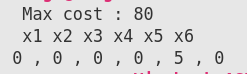
\includegraphics[]{10.png}
    \centering
    \caption{Результат работы программы}
\end{figure}
